\chapter{Resultados}
\label{chap:resultados}

%\endinput

\section{Introducci\'on}
En este cap\'itulo se presentan los distintos escenarios que fueron planteados para la verificaci\'on de los procesos y el an\'alisis de los resultados.\\

Dado que para la metodolog\'ia de estimaci\'on de errores que proponemos, utilizamos datos reales de una misi\'on operativa argentina, hubiera sido
deseable contar con datos de alertas de colisiones reales propios de esa misi\'on, ya que esto hubiera permitido hacer una validaci\'on end-to-end de todo el prototipo. No obstante, por cuestiones de confidencialidad, no fue posible tener acceso a esa informaci\'on.
Frente a este panorama, se detalla a continuaci\'on la secuencia de etapas de validaci\'on que permiten evaluar, cada una de las instancias del procesamiento.\\

En primer lugar fue fundamental corroborar las propagaciones de los TLE realizadas con la librer\'ia de python {\it{sgp4-1}} \citep{sgp4python}, para ello utilizamos la versi\'on de prueba que ofrece el software STK: {\it{System Tool Kit}}, \citep{stk}.\\

Para la validaci\'on de los resultados de la implementaci\'on del m\'etodo de Osweiler en la generaci\'on de matrices de covarianza, se compararon los resultados de ARxCODE para dos de los escenarios que se publican en el trabajo.\\

El m\'etodo que se propone para la estimaci\'on de la propagaci\'on de errores, es el que m\'as dificultades present\'o para ser validado. Al basarse plenamente en los datos de la misi\'on cuyos resultados de colisi\'on de alerta no pudieron ser suministrados, fue analizado en comparaci\'on con resultados estad\'isticos globales, o sobre el estudio de encuentros de otras misiones.\\

Los resultados de las matrices de covarianza calculadas y la estimaci\'on de la m\'inima distancia, fueron comparadas con la informaci\'on de correos electr\'onicos de alerta y CDM de acceso p\'ublico.\\

Finalmente la implementaci\'on del c\'alculo de probabilidad de colisi\'on fue evaluada analizando diez casos de prueba que contienen el dato de la PoC: cuatro casos publicados mediante el servicio web de SOCRATES \citep{Kelso} que ofrece Celestrack (Tabla \ref{tab:sisal}),  dos casos  presentados en el libro de Klinkrad \citep{KlinkradChapter8} y cuatro casos publicados en un trabajo de Xu-Xiong \citep{xu2014method}. \\

\section{Implementaci\'on del modelo SGP4 en Python}

Para la propagaci\'on de las posiciones orbitales con el modelo SGP4 (Sec. \ref{subsec:sgp4model}) utilizamos la librer\'ia de python {\bf{sgp4-1}} \citep{sgp4python}.
Luego usamos el software STK para comparar nuestras propagaciones y asegurarnos la correcta utilizaci\'on y configuraci\'on de la librer\'ia sgp4-1.\\

Las Tablas \ref{tab:arcode}  y \ref{tab:stk} muestran las efem\'erides de la misi\'on operativa durante los primeros cuatro minutos del d\'ia 01/01/2013.
Ambas fueron generadas a partir del mismo TLE y presentan resultados que difieren en algunos metros para los peores casos. Resultado aceptable, teniendo en cuenta que las estimaciones groseras de errores para las propagaciones hechas con TLEs y SGP4 acarrean errores de kil\'ometros o decenas de kil\'ometros.\\

% \underline{TLE.}
% {\small
% \begin{verbatim}
% 1 xxxxU xxxxx   13001.74853505  .00000428  00000-0  75550-4 0  9996
% 2 xxxxx 098.0122 011.5654 0001526 107.5603 009.0604 14.72289948 84036
% \end{verbatim}}


\begin{table}[!h]
\caption{Resultados que genera ARxCODE utilizando la librer\'ia sgp4 de python para la propagaci\'on.}
\centering
\resizebox{17cm}{!}{
\begin{tabular}{lcccccc}
\hline
Epoca & x [km] & y [km] & z [km] & vx $[km/s]$ & vy $[km/s]$ & vz $[km/s]$\\
\hline
2013-01-01 00:00&-2372.76245& -1381.01830& 6465.57494& -6.95099& -0.93631& -2.74523\\
2013-01-01 00:01& -2784.64672& -1434.31269& 6287.6158& -6.77374& -0.83955& -3.18470\\
2013-01-01 00:02& -3185.05363& -1481.69530& 6083.67196& -6.56854& -0.73932& -3.61109\\
2013-01-01 00:03& -3572.3305& -1522.96975& 5854.58154& -6.336229& -0.63602& -4.02263\\
2013-01-01 00:04& -3944.8780& -1557.96472& 5601.28702& -6.077737& -0.53007& -4.417616\\
\hline
\label{tab:arcode}
\end{tabular}
}
\end{table}

\begin{table}[!h]
\caption{Resultados del Systems Tool Kit (STK) propagando el mismo TLE que ARxCODE.}
\centering
\resizebox{17cm}{!}{
\begin{tabular}{lcccccc}
\hline
\'Epoca & x [km] & y [km] & z [km] & vx [km/s] & vy [km/s] & vz [km/s]\\
\hline
2013-01-01 00:00&-2372.76302&-1381.02018&6465.57433&-6.95099&-0.93631&-2.74523\\
2013-01-01 00:01&-2784.64726&-1434.31473&6287.61518&-6.77374&-0.83955&-3.18470\\
2013-01-01 00:02&-3185.05413&-1481.69750&6083.67116&-6.56854&-0.73932&-3.61109\\
2013-01-01 00:03&-3572.33097&-1522.97210&5854.58064&-6.33622&-0.63602&-4.02263\\
2013-01-01 00:04&-3944.87849&-1557.96721&5601.28604&-6.07773&-0.53008&-4.41761\\
\hline
\label{tab:stk}
\end{tabular}
}
\end{table}


%\textcolor{red}{hacer las diferencias medias para todo un dia en python y publicarlas}

\section{Estudio de errores de TLE con datos hist\'oricos}

El trabajo de Osweiler publica los resultados de las matrices de covarianza generadas, para 6 misiones y 8 ventanas de tiempo.\\

Para la validaci\'on se tomaron dos escenarios muy diferentes en cuanto a la altura del sat\'elite: LAGEOS-1 a m\'as de $5000$ km y ICESAT a $600 $ km, (Tabla \ref{tab:satescenarios}).\\


\begin{table}[!h]
\caption[Sat\'elites de Estudio]{Resumen de las caracter\'isticas de los sat\'elites a analizar.}

      \begin{tabular}{cccccc}
      \hline
      Nombre & ID NORAD & Altura & Ecc. & Inclinaci\'on & B* \\
      \hline
      LAGEOS-1 & 8820 & $5850$ & $0.004$ & $109.8$ & $0.0001$ \\
      ICESAT & 27642 & $600$ & $0.0002 - 0.001$ & $94$ & var\'ia \\
      \hline
      \end{tabular}
    \label{tab:satescenarios}
\end{table}

Se presentan a continuaci\'on las tablas con los resultados comparativos, entre los valores publicados (Tablas \ref{tab:icesatOSW} y \ref{tab:lageosOSW}) y los valores obtenidos por ARxCODE (Tablas \ref{tab:icesatARX} y \ref{tab:lageosARX}) para una \'unica ventana temporal.\\

Puede apreciarse, que los errores son muy grandes para el ICESAT, de baja altura, que se ve m\'as perturbado por el efecto atmosf\'erico, que no es modelable con precisión; mientras que el LAGEOS-1 presenta errores muchos \'ordenes de magnitud menor.\\

\subsection*{Tablas comparativas ICESAT}

\begin{table}[!h]
\centering
\makebox[0pt][c]{\parbox{1.0\textwidth}{%
    \begin{minipage}[t]{0.48\hsize}
    \caption{Matriz de Covarianza. \citep{osweiler} \\ ICESAT del 1-Mar-03 al 16-Mar-03.}
     \resizebox{8cm}{!}{
    \begin{tabular}{cccc}
      \hline
    Vent 1 & $R_{v}$ (km) & $R_{n}$ (km) & $R_{c}$ (km)\\
    \hline
    $R_{v}$ &  2667.377375  &    27.248658   &   -8.22221222\\
    $R_{n}$ & 27.248658  &   0.34323269 & -0.12314379\\
    $R_{c}$ & -8.22221222 & -0.12314379 & 0.07316443\\
    \hline
    \end{tabular}}
      \label{tab:icesatOSW}
    \end{minipage}
    \begin{minipage}[t]{0.48\hsize}
    \caption{Matriz de Covarianza de ARxCODE. \\ ICESAT del 1-Mar-03 al 16-Mar-03.}
    \resizebox{8cm}{!}{
      \begin{tabular}{cccc}
	\hline
      Vent 1 & $R_{v}$ (km) & $R_{n}$ (km) & $R_{c}$ (km)\\
      \hline
      $R_{v}$ &  2667.37364259 &   27.2488814  &   -8.22232626\\
      $R_{n}$ & 27.2488814  &  0.3432413 &  -0.12314867\\
      $R_{c}$ & -8.22232626 & -0.12314867 &  0.073167\\
      \hline
      \end{tabular}}
        \label{tab:icesatARX}
    \end{minipage}
 %   \hfill
}}
\end{table}

\begin{table}[!h]
\caption{Diferencias de ARxCODE respecto a Osweiler \citep{osweiler}}

  \begin{tabular}{cccc}
  \hline
 Vent 1 & Dif.$R_{v}$ (km) & Dif.$R_{n}$ (km) & Dif.$R_{c}$ (km)\\
 \hline
 Dif. $R_{v}$ & -0.00373241 & 0.0002234 & -0.00011404 \\
 Dif. $R_{n}$ &  0.0002234 &  0.000008 & -0.000004\\
 Dif. $R_{c}$ & -0.00011404  & -0.000004 &  0.000002\\
 \hline
 \end{tabular}
 \label{tab:icesatcomp}
\end{table}


\subsection*{Tablas comparativas LAGEOS-1}

\begin{table}[!h]
\centering
\makebox[0pt][c]{\parbox{1.0\textwidth}{%
    \begin{minipage}[b]{0.48\hsize}
    \caption{Matriz de Covarianza. \citep{osweiler} \\ LAGEOS-1 del 1-Mar-03 al 16-Mar-03}
    \resizebox{8cm}{!}{
      \begin{tabular}{cccc}
	\hline
      Vent 1 & $R_{v}$ (km) & $R_{n}$ (km) & $R_{c}$ (km)\\
      \hline
      $R_{v}$ &  0.37863904 & -0.03440871 & 0.02772177 \\
      $R_{n}$ & -0.03440871 & 0.00401173 & -0.00272334 \\
      $R_{c}$ & 0.02772177 & -0.00272334 & 0.00843443\\
      \hline
      \end{tabular}}
        \label{tab:lageosOSW}
    \end{minipage}
    \hfill
    \begin{minipage}[b]{0.48\hsize}
    \caption{Matriz de Covarianza de ARxCODE \\ LAGEOS-1 del 1-Mar-03 al 16-Mar-03}
     \resizebox{7.5cm}{!}{
    \begin{tabular}{cccc}
      \hline
    Vent 1 & $R_{v}$ (km) & $R_{n}$ (km) & $R_{c}$ (km)\\
    \hline
    $R_{v}$ & 0.378619 & -0.0343598 & 0.02771527 \\
    $R_{n}$ & -0.0343598 &  0.004002 & -0.0027171 \\
    $R_{c}$ & 0.02771527 & -0.0027171 &  0.0084302 \\
    \hline
    \end{tabular}}
      \label{tab:lageosARX}
   \end{minipage}
    \hfill
}}
\end{table}

\begin{table}[!h]
\caption{Diferencias de ARxCODE respecto a Osweiler, \citep{osweiler}.}
 \begin{tabular}{cccc}
  \hline
 Vent 1 & Dif.$R_{v}$ (km) & Dif.$R_{n}$ (km) & Dif.$R_{c}$ (km)\\
 \hline
 Dif. $R_{v}$ & 0.000020 &  -0.000048 &  0.000006 \\
 Dif. $R_{n}$ & -0.000048 &   0.000009 &  -0.000006 \\
 Dif. $R_{c}$ & 0.000006 &  -0.000006 &   0.000004 \\
 \hline
 \end{tabular}
 \label{tab:lageoscomp}
\end{table}

Las diferencias que resultan en la comparaci\'on con los resultados que arroja ARxCODE, son todas menores a los metros (Tablas \ref{tab:icesatcomp} y \ref{tab:lageoscomp}). En particular LAGEOS muestra errores menores que ICESAT, ya que al ser un sat\'elite a mayor altura, el efecto atmosf\'erico es menor y el modelo de propagaci\'on, se adapta mejor.\\

\subsection*{Diferencias de los escenarios iterando el TLE primario en el m\'etodo de Osweiler}
Estudio hecho sobre los errores que se producen en las propagaciones de los TLE en funci\'on de la cantidad de d\'ias que se propaguen.\\

Estos resultados ofrecen mayor informaci\'on respecto a los errores que se cometen en funci\'on de la cantidad de d\'ias que se propagan los TLE.\\

Para la generaci\'on de los datos, se propagaron todos los TLE del conjunto hacia las fechas de todos los TLE con fechas m\'as actualizadas, dentro del conjunto (Fig. \ref{fig:todosOSW}). Las diferencias que resultaron se plasman en funci\'on del intervalo de propagaci\'on, en las Figuras \ref{fig:icesatTot} y \ref{fig:lageosTot} para el ICESAT y el LAGEOS respectivamente. 

\begin{figure}[!h]
\centering
  \textbf{Propagaci\'on y comparaci\'on de TLE }\par\medskip
  \fbox{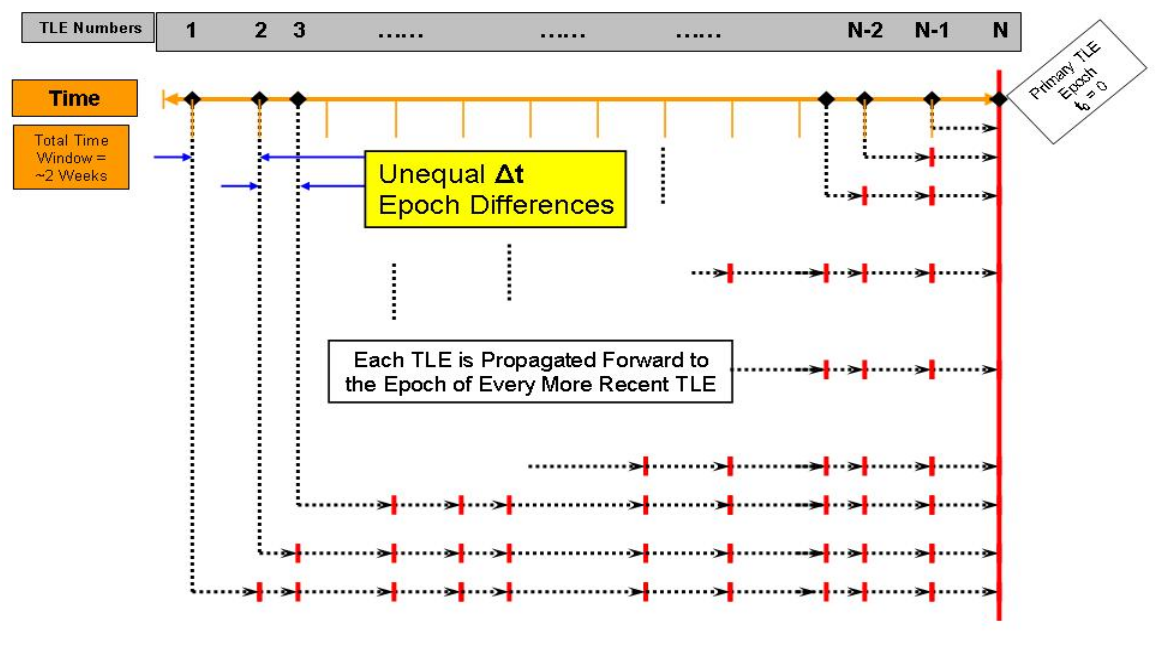
\includegraphics[width=0.8\textwidth]{imagenes/todosOSW}}
  \caption{Esquematizaci\'on del algoritmo para comparar la propagaci\'on de cada TLE del set hacia fechas futuras de los TLE del set. Extra\'ido del trabajo de Osweiler, \citep{osweiler}}.
  \label{fig:todosOSW}
\end{figure}

\begin{figure}[h!]
\centering
  \subfigure[Diferencias ICESAT - ARxCODE]{
    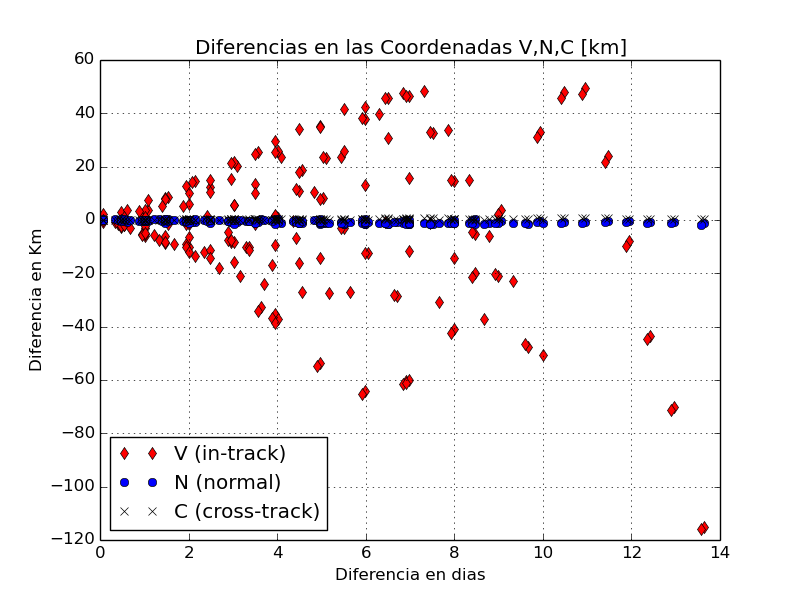
\includegraphics[width=0.48\textwidth]{imagenes/TLEdifTot27642esc52}
  }
  \subfigure[Diferencias ICESAT - Osweiler, \citep{osweiler}]{
    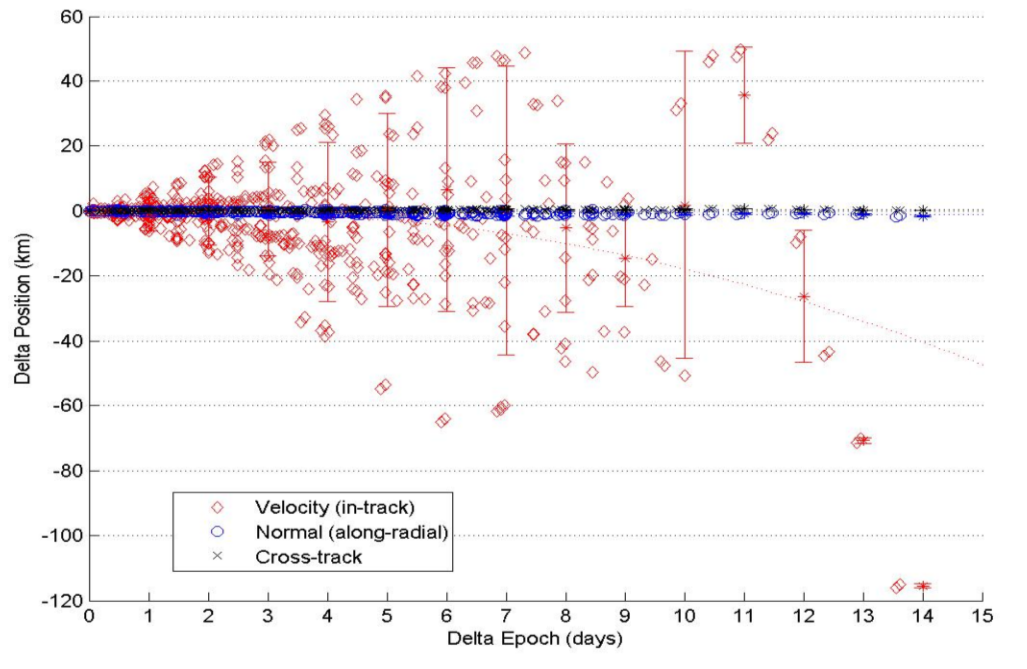
\includegraphics[width=0.48\columnwidth, keepaspectratio]{imagenes/ICESATdifTot}
  }
  \caption{Gr\'afico con Diferencias Totales del escenario ICESAT}
  \label{fig:icesatTot}
\end{figure}

\begin{figure}[h!]
\centering
  \subfigure[Diferencias LAGEOS-1 - ARxCODE]{
    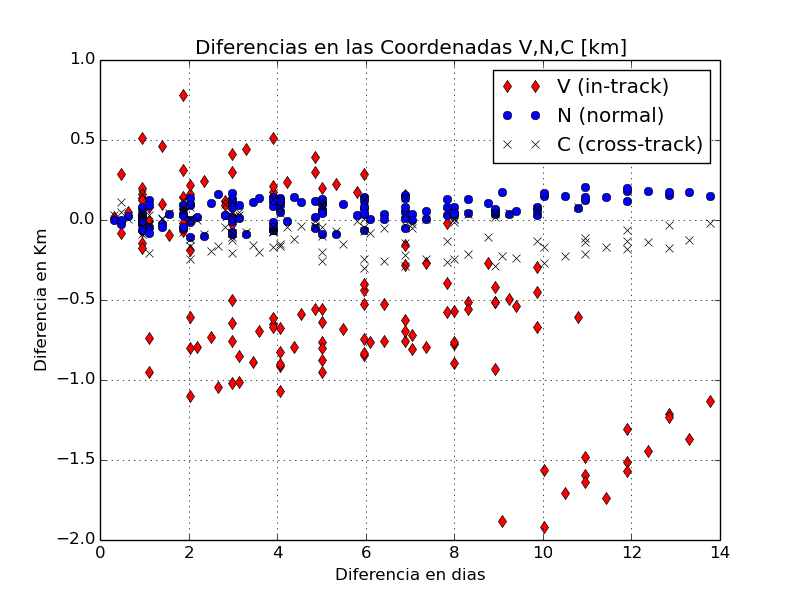
\includegraphics[width=0.48\textwidth]{imagenes/TLEdifTot8820esc11}
  }
  \subfigure[Diferencias LAGEOS-1 - Osweiler, \citep{osweiler}]{
    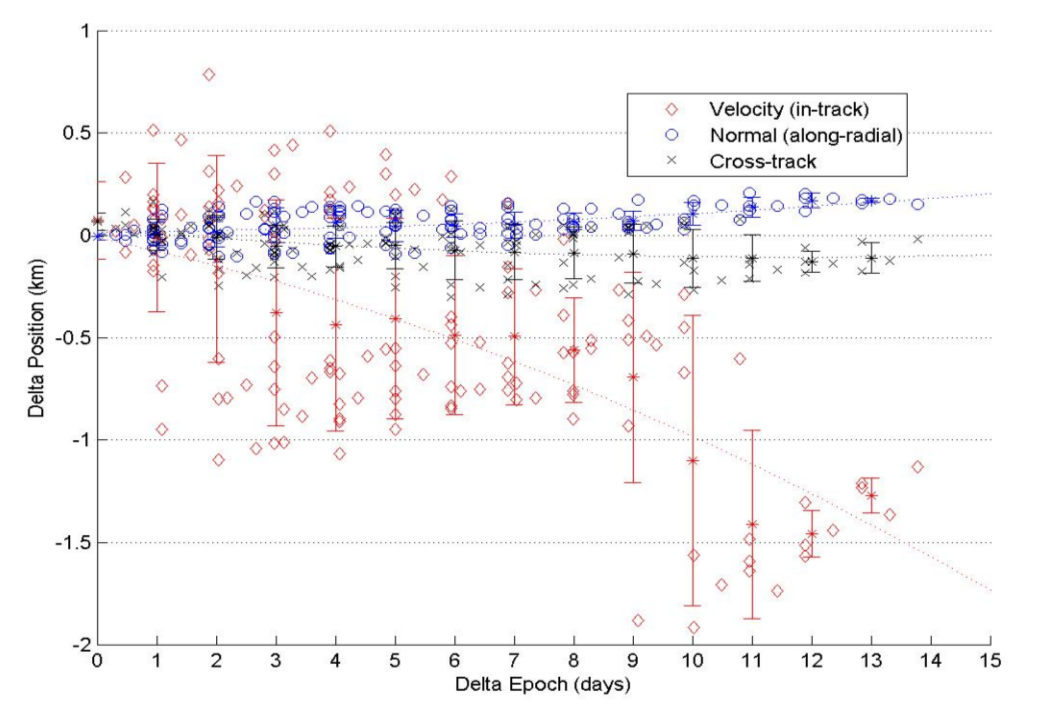
\includegraphics[width=0.48\columnwidth, keepaspectratio]{imagenes/LAGEOSdifTot}
  }
  \caption{Gr\'afico con Diferencias Totales del escenario LAGEOS-1}
  \label{fig:lageosTot}
\end{figure}

Los errores que se observan en la propagaci\'on de TLE, en funci\'on de la cantidad de d\'ias propagados, muestran comportamientos casi id\'enticos.\\

En este estudio, puede apreciarse una clara diferencia en las cotas de los errores, siendo el sat\'elite ICESAT, de menor altura el que muestra errores mayores en un rango de -120 a 60 km, mientras que el LAGEOS, contiene las diferencias entre -2 y 1 km.\\

No obstante, en ambos se distingue, que la componente asociada a la velocidad (V {\it{in-track}}) es la que mayor error acumula en propagaciones m\'as largas. Esto se debe a que el modelo es d\'ebil en cuanto a la perturbaci\'on que introduce la atm\'osfera, directamente vinculada a la velocidad de los objetos para el caso del ICESAT o en cuanto al modelo que describe la presi\'on de radiaci\'on solar en el caso del LAGEOS.\\

Se concluye a partir de esta secci\'on, que ARxCODE implementa el m\'etodo de Osweiler y la construcci\'on de las diferencias de pares correctamente. 

\section{Estudio de errores de TLE con efem\'erides precisas}
\subsection*{Sistema de referencia TOD}
En esta secci\'on se muestran los resultados de comparar las posiciones obtenidas utilizando TLE y realizando las propagaciones con SGP4, contra las efem\'erides precisas.\\ 

En primer lugar fue necesario plasmar las posiciones en el mismo sistema de referencia, ya que los productos del departamento de din\'amica orbital con los que trabajamos ofrecen las posiciones orbitales en el sistema de referencia verdadero de la fecha \ac{TOD}, mientras que los resultados de las propagaciones con el SGP4 se encuentran en el sistema \ac{TEME}. Para poder hacer comparaciones desarrollamos un m\'odulo que transforma las coordenadas y velocidades, del sistema TEME al sistema TOD (Ap\'endice. \ref{App1}).\\

Para la validaci\'on del mismo, se utilizaron TLE de la misi\'on y se los propagaron con el SGP4. Los resultados se transformaron al sistema TOD con el m\'odulo desarrollado y luego fueron comparados con los productos del STK, corridos para el mismo TLE y publicados en el sistema TOD. Se obtuvieron diferencias menores a los mil\'imetros, (Tabla \ref{tab:compprecisas}).\\

\begin{table}[!h]
\caption{Comparaci\'on entre ARxCODE y STK de \\la transformaci\'on de TEME a TOD.}
\begin{tabular}{l|c}
  \hline
  Coordenada  X &  0.0003168 [m]\\
  Coordenada Y &  0.0006370 [m]\\
  Coordenada Z &  0.0005133 [m]\\
  \hline
\end{tabular}
\label{tab:compprecisas}
\begin{flushleft}
\small 1 de Enero de 2013, paso 1 minuto.
\end{flushleft}
\end{table}

\subsection*{Estad\'istica de Errores}
Con la certeza de que los datos eran compatibles y pod\'ian ser comparados (ambos se ubican en el sistema TOD), se inici\'o el procesamiento de comparaci\'on de las posiciones de las efem\'erides precisas de la misi\'on y las propagaciones de los TLE, para la estimaci\'on de los errores de la propagaci\'on, (Sec. \ref{subsec:errorProp}).\\

En un pre-procesamiento sobre un periodo amplio de la misi\'on, constatamos que fuera de los intervalos de maniobras por {\it{commissioning}}\footnote{Puesta en \'orbita nominal} o maniobras de rutina, los TLE presentan un error que es {\it{acotado}}, {\it{estable}} y/o modelable. \\

Se realizaron comparaciones para todo el a\~no 2012 y todo el a\~no 2013. En ambos casos los resultados del estudio mostraron el comportamiento esperado, con errores m\'aximos del orden de las decenas de kil\'ometros (Fig. \ref{fig:sacd2012} y \ref{fig:sacd2013}).\\

\begin{figure}[!h]
\centering
  \textbf{Tendencia Anual 01/01/2012 - 30/08/2012}\par\medskip
  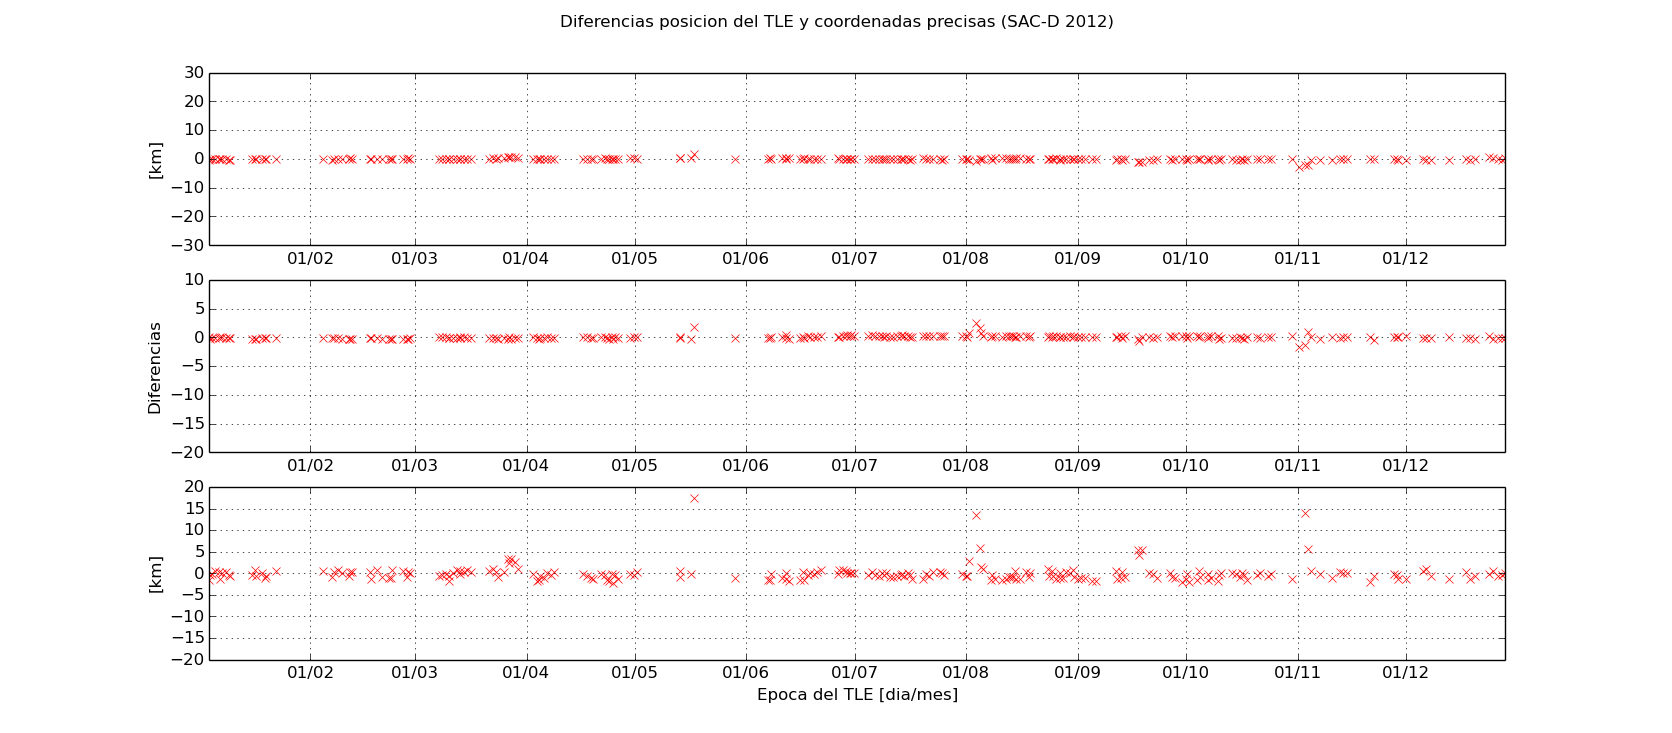
\includegraphics[width=\textwidth]{imagenes/sacDtendencia2012}
  \caption{Diferencias en las posiciones propagadas durante el a\~no 2012 y las efem\'erides precisas generadas por CODS [Sistema TOD]}
  \label{fig:sacd2012}
\end{figure}


\begin{figure}[H]
\centering
  \textbf{Tendencia Anual 01/01/2013 - 30/08/2013}\par\medskip
  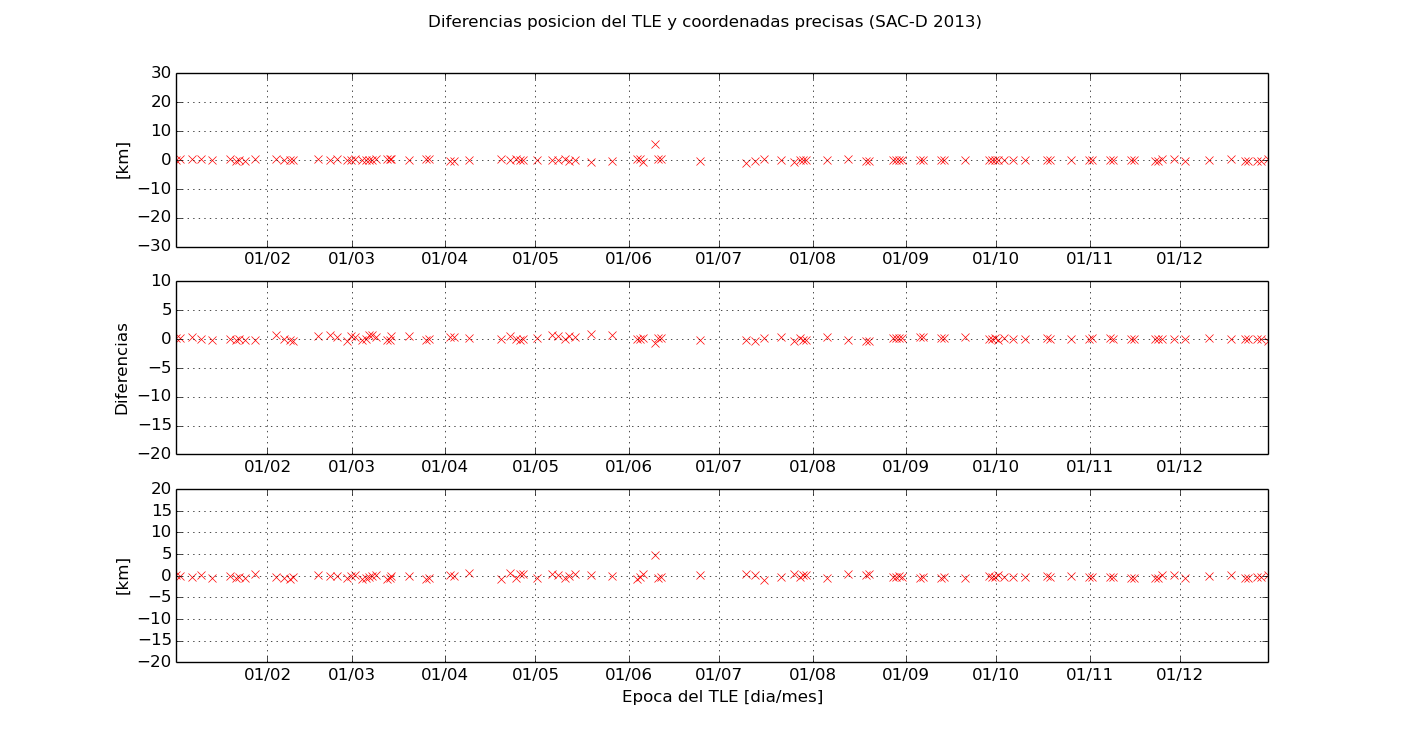
\includegraphics[width=\textwidth]{imagenes/sacDtendencia2013}
  \caption{Diferencias en las posiciones propagadas durante el a\~no 2013 y las efem\'erides precisas generadas por CODS [Sistema TOD]}
  \label{fig:sacd2013}
\end{figure}

\subsection*{Generaci\'on de la tabla de propagaci\'on de errores}

Como se explic\'o en la Sec. \ref{subsec:errorProp}, para estimar los errores en la propagaci\'on se propone un m\'etodo que utiliza una tabla (Tabla \ref{tab:resultatabla}), generada a partir de la estad\'istica que resulta de comparar las propagaciones de los TLE de la misi\'on operativa, con las efem\'erides precisas. Las comparaciones se hacen en el periodo de Enero a Diciembre del a\~no 2013, en intervalos de 1 a 6 d\'ias, con paso 1 segundo.

\begin{table}[!h]
\caption[Tabla con los valores medios para la propagaci\'on de errores.]{Valores medios de las varianzas calculadas\\ para la propagaci\'on de errores.\\ Autor\'ia propia.}
\begin{tabular}{lccc}
\hline \hline
\rowcolor{yellow!35}
&$\sigma^{2}_R [km]$ &$\sigma^{2}_T [km]$ &$\sigma^{2}_N [km]$\\
\hline \hline
< 1 d\'ia & 0.052& 0.644& 0.138\\
\hline
1 d\'ia & 0.038& 0.450& 0.142\\
\hline
2 d\'ias & 0.027& 0.408& 0.148\\
\hline
3 d\'ias & 0.019& 0.384& 0.155\\
\hline
4 d\'ias & 0.014& 0.374& 0.165\\
\hline
5 d\'ias & 0.013& 0.377& 0.179\\
\hline
6 d\'ias & 0.015& 0.399& 0.196\\
\hline
\end{tabular}
\label{tab:resultatabla}
\end{table}

Los resultados que se encuentran, no es posible validarlos directamente. No obstante, son comparables a los que proponen Flohrer et al., \citep{flohrer2008assessment}, en la {\it{lookup table}} generada considerando todos los objetos del cat\'alogo al 01 de Enero de 2008 (Fig.  \ref{fig:flohrer}). Los valores de las desviaciones est\'andar que resultan del m\'etodo propuesto son menores casi en un orden de magnitud en la componente R y de igual orden en T y N en relaci\'on a los valores correspondientes a las tablas gen\'ericas que publican Flohrer et al., \citep{flohrer2008assessment}. Puede concluirse que el escenario de la misi\'on SAC-D est\'a contenido en la estad\'istica que refleja el trabajo de Flohrer. 

\begin{figure}[!h]
  \centering
  \fbox{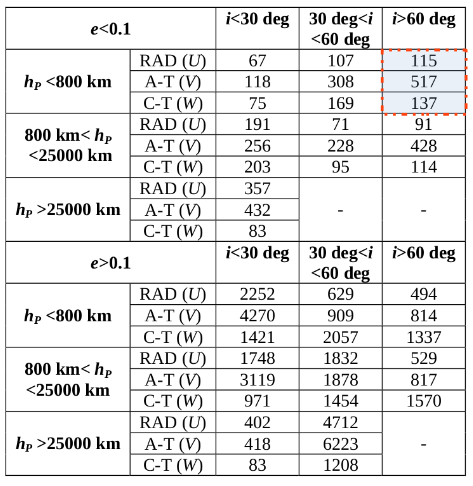
\includegraphics[width=0.5\textwidth]{imagenes/flohrertabla}}
  \caption{{\it{Look-up table}} [metros] de los resultados promediados del an\'alisis del cat\'ologo completo al 1 de enero de 2008, de los errores en las coordenadas UVW, clasificados por excentricidad, inclinaci\'on y altura. Se resaltan en celeste las celdas correspondientes a la configuraci\'on de la misi\'on operativa que se utiliz\'o en este trabajo. Extra\'ido de Flohrer et al., \citep{flohrer2008assessment}}.
  \label{fig:flohrer}
\end{figure}

% \begin{itemize}
%  \item Klinkrad Tabla para 14 misiones.
%  \item Paper del research gate
%  \item Peterson?!
% \end{itemize}
% 
% FINALIZAR CON COMPARACI\'ON TLE vs TLE. 

\section{C\'alculo de la Probabilidad de Colisi\'on}

Hasta este punto, se han validado cada uno de los procesos por separado.
Resta hacer pruebas que involucren todo el procedimiento, es decir, identificar los objetos y el TCA y correr los procesamientos de ARxCODE hasta obtener los valores de la PoC.
A tal fin, fue necesario conseguir registros que contuvieran la informaci\'on completa de una situaci\'on de encuentro.\\

\subsection*{Casos de Prueba}
Por un lado se consiguieron correos electr\'onicos de alerta p\'ublicos en internet, y por otro CDM tambi\'en p\'ublicos\footnote{https://cwe.ccsds.org/moims/docs/Forms/AllItems.aspx?RootFolder=\%2Fmoims\%2Fdocs\%2FMOIMS-NAV\%2FDraft\%20Documents\%2FConjunction\%20Data\%20Message\%20\%28CDM\%29}, pero ninguno de esos datos se corresponden con la misi\'on operativa, cuyas efem\'erides precisas analizamos y utilizamos en la construcci\'on del modelo estad\'istico de propagaci\'on de errores.
As\'i mismo, ni los correos encontrados ni los CDM descargados contienen informaci\'on de la PoC asociada al encuentro. 

Formato de los {\bf{correos electr\'onicos}}:\\
\begin{center}
\fbox{\parbox[b]{0.8\linewidth}{\small{
The United States Joint Space Operations Center (JSpOC) has identified a\\
predicted conjunction between DELFI C3 (SCC\# 32789) and SCC\# 23657.\\

Primary Object: DELFI C3 (SCC\# 32789)\\
Secondary Object: SCC\# 23657\\
Time of Closest Approach: 15 JUL 2012 21:21 UTC \\

Overall miss distance: 760 meters\\
Radial (dU) miss distance: -186 meters\\
In-Track (dV) miss distance: -389 meters\\
Cross-track (dW) miss distance: -626 meters\\

Primary Radial Error (U): 38 meters\\
Primary In-track Error (V): 1388 meters\\
Primary Cross-track Error (W): 11 meters\\

Secondary Radial Error (U): 8 meters\\
Secondary In-track Error (V): 338 meters\\
Secondary Cross-track Error (W): 2 meters\\}
}}\label{box:mail}
\end{center}


La Figura \ref{fig:tablamails}, muestra el resumen de la informaci\'on de todos los correos electr\'onicos que fueron procesados con ARxCODE. \\

\begin{figure}[!h]
  \centering
  \fbox{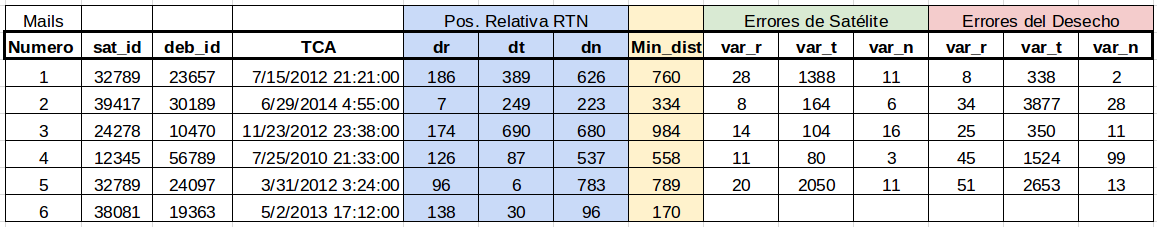
\includegraphics[width=\textwidth]{imagenes/tablamails}}
  \caption{Contenido de los correos electr\'onicos utilizados para comparar los resultados.}
  \label{fig:tablamails}
\end{figure}

Se listan a continuaci\'on los seis CDM cuyos datos fueron procesados con ARxCODE (Fig. \ref{fig:cdmsproc}). 

 \begin{figure}[H]
  \centering
  \fbox{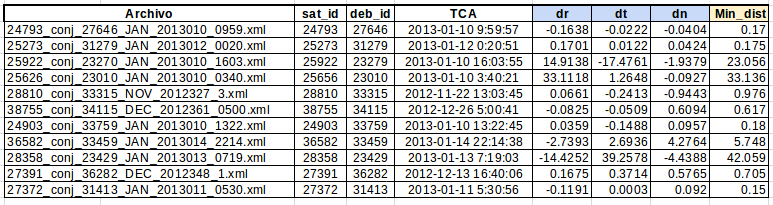
\includegraphics[width=\textwidth]{imagenes/tablaCDM}}
  \caption{Contenido de los CDM utilizados para comparar los resultados.}
  \label{fig:cdmsproc}
\end{figure}

Por \'ultimo se analizaron diez casos de prueba que contienen el dato de la PoC: cuatro casos publicados mediante el servicio web de SOCRATES \citep{Kelso} que ofrece Celestrack (Tabla \ref{tab:sisal}),  dos casos  presentados en el libro de Klinkrad \citep{KlinkradChapter8} y cuatro casos publicados en un trabajo de Xu-Xiong \citep{xu2014method}.\\

Como se mencion\'o en la Introducci\'on (Sec. \ref{sec:antecedentes}), SOCRATES es un 
servicio web v\'ia Celestrack.com, mantenido por el CSSI (Center for Space Standards \& Innovation) de la agencia AGI: Analytical Graphics, Inc. El mismo ofrece informaci\'on de los acercamientos de riesgo futuros. Se pueden solicitar los acercamientos que involucran a las misiones que son de inter\'es para uno y SOCRATES lista las 10 situaciones m\'as cr\'iticas para los d\'ias futuros. En este caso se han seleccionado sat\'elites con \'orbitas bajas, de observaci\'on de la Tierra, a saber: SentinelB1 (41456), Cosmos-Skymed3 (33412) y Envisat (27386) (Tabla \ref{tab:escenariosSOCRATES}).

\begin{table}[!h]
 \caption{Casos de Prueba tomados del servicio SOCRATES (Celestrack.com).}
\resizebox{13cm}{!}{
\begin{tabular}{lccccccc}
 \hline \hline
  \rowcolor{lightgray}
 \# & sat id & deb id & TCA & Min Dist [km] & PoC  \\
 \hline
 1 & 41456 & 35732 & 29-06-2018 22:22:48.14 & 0.039 & 1.74e-03 \\
 2 & 33412 & 19008 & 30-06-2018 03:42:30.937 & 0.096 & 2.62e-04\\
 3 & 27386 & 35519 & 25-05-2018 09:46:17.533 & 0.926 & 1.10e-04\\
 4 & 27386 & 37887 & 08-07-2018 23:36:38.326 & 0.137 & 6.10e-04\\
 \hline
\end{tabular} }
\label{tab:escenariosSOCRATES}
\end{table}

En el cap\'itulo ocho de su libro, Klinkrad \citep{Klinkrad}, publica una tabla que contiene siete situaciones de encuentros de riesgo para las misiones ENVISAT y ERS-2. De esos escenarios s\'olo se han podido reproducir dos, ya que no fue posible identificar los c\'odigos de NORAD de los desechos involucrados en el resto de los encuentros (Tabla \ref{tab:escenariosKlinkrad}).

\begin{table}[!h]
 \caption{Casos de prueba tomados del libro de Klinkrad \citep{Klinkrad}.}
\resizebox{13cm}{!}{
\begin{tabular}{lccccccc}
 \hline \hline
  \rowcolor{lightgray}
\# & sat id & deb id & TCA & Min Dist [km] & PoC  \\
 \hline
 5 & 27386 &  12442 & 2004-09-02 19:14:11 & 1.297& 2.186e-04\\
 6 & 23560 &  16681 & 2004-09-29 23:56:02 & 0.067& 1.546e-04\\
 \hline
\end{tabular} }
\label{tab:escenariosKlinkrad}
\end{table}

En un mismo sentido, se utilizaron los valores publicados en el trabajo de Xu y  Xiong, \citep{xu2014method}, donde  se presentan las estimaciones de la m\'inima distancia y la Poc, utilizando un m\'etodo general y el m\'etodo desarrollados por ellos (Tabla \ref{tab:escenariosxx}).\\

\begin{table}[H]
\caption{Casos de prueba tomados del trabajo de  Xu \& Xiong \citep{xu2014method}.}
\resizebox{15cm}{!}{
\begin{tabular}{lcccccccc}
 \hline \hline
  \rowcolor{lightgray}
\# & sat id & deb id & TCA & Min Dist [km] & PoC (general) & PoC \\
 \hline
 7  & 25415 & 31445 & 2013-03-18 14:44:34 & 0.115 & 1.24e-05  & 1.52e-05\\
 8  & 20737 & 20738 & 2013-03-17 10:39:31 & 0.104 & 1.706e-06 & 2.15e-06\\
 9  & 27939 & 31588 & 2013-03-16 13:46:21 & 0.098 & 3.01e-05  & 3.51e-05 \\
 10 & 11308 & 32315 & 2013-03-15 03:02:16 & 0.094 & 1.8e-05   & 2.05e-05\\
 \hline
\end{tabular} }
\label{tab:escenariosxx}
\end{table}

\subsection*{Implementaci\'on de los algoritmos de c\'alculo de PoC}
En este trabajo se utilizaron tres m\'etodos distintos para estimar el valor de la PoC. El primero de ellos, que denominamos {\it{m\'etodo del l\'imite}}, es una simple expresi\'on que resulta como conclusi\'on de un trabajo de Alfano \citep{alfano2008method}, y dado que resulta una implementaci\'on muy sencilla no realizamos ninguna prueba para evaluarla.

El segundo de los m\'etodos es el que propone Lei-Chen \citep{leichen}. Tambi\'en consiste en una simple expresi\'on pero el resultado puede compararse con la resoluci\'on de la integral num\'erica que el m\'etodo aproxima. A su vez las variables que se introducen en la ecuaci\'on deben ser previamente transformadas al sistema de referencia RSW. En este caso fue posible aprovechar un ejemplo que el propio Lei-Chen incorpora en su libro para verificar los dos puntos mencionados y por ende la correcta implementaci\'on del algoritmo.

\subsubsection*{M\'etodo de Lei-Chen: validaci\'on con la resoluci\'on de la integral}
Se toman como datos iniciales, los valores publicados por el propio autor Lei-Chen, \citep{leichen}, y se calcula la PoC, tanto para la expresi\'on anal\'itica como para la integral. Para esta \'ultima se utiliza la librer\'ia {\it{scipy.integrate}}  de Python.\\

De las expresiones para el c\'alculo de la PoC (Eq. \ref{eq:pocintegral} y Eq. \ref{eq:pocexpress}), se desprende que ser\'an necesarios los datos: ($\mu_{x}, \mu_{y}$), ($\sigma_{x}, \sigma_{y}$), $r_{a}$.\\

Se tomaron los datos que utiliza Lei-Chen en el ejemplo para el caso de las \'orbitas circulares y se calcul\'o la PoC a partir de la expresi\'on expl\'icita y realizando la integral.\\

\begin{minipage}[t]{0.28\textwidth}
{\bf{Valores iniciales.}}\\

\begin{tabular}{|lc|}
\hline
 Dato & valor \\
\hline
$\mu_{x}$ & 0.031731 [km]\\
$\mu_{y}$ & 0.697294 [km]\\
$\sigma_{x}$ & 0.0430576\\
$\sigma_{y}$ & 0.2941297\\
$r_{a}$ & 0.01 [km]\\
\hline
\end{tabular}
\end{minipage}
\begin{minipage}[t]{0.7\textwidth}
\begin{mdframed}[
        linecolor=red,linewidth=2pt,% 
        frametitlerule=true,% 
        apptotikzsetting={\tikzset{mdfframetitlebackground/.append style={%
            shade,left color=white, right color=blue!20}}}, 
        frametitlerulecolor=blue,
        frametitlerulewidth=1pt, innertopmargin=\topskip,
        frametitle={Probabilidad de Colisi\'on},
        outerlinewidth=1.25pt
    ]
\large
\captionof{table}{Resultados Comparativos del c\'alculo de la PoC.}
\begin{tabular}{|l|l|l|}
  \hline
 Te\'orico & Expresi\'on & Valor de la Integral\\
 \hline
 1.8079750e-04 & 1.8079124e-04 & 1.8071110e-04\\
 \hline
\end{tabular}
\label{tab:poccomp}
\end{mdframed}
\end{minipage}

\vspace{0.5cm}
Como se observa en el recuadro de las probabilidades de colisi\'on (Tabla \ref{tab:poccomp}); las f\'ormulas implementadas coinciden con el valor de la bibliograf\'ia hasta el cuarto d\'igito significativo de la expresi\'on.\\

En este punto se confirma que, una vez que se obtienen: $\mu_{x}$, $\mu_{y}$, $\sigma_{x}$, $\sigma_{y}$ y el radio de colisi\'on $r_{a}$, ya puede calcularse la PoC. 
Ahora resta verificar, paso a paso c\'omo llegar de los inputs de ARxCODE, a estos par\'ametros que se introducen en las ecuaciones. \\

\subsubsection*{M\'etodo de Lei-Chen: validaci\'on de la transformaci\'on al sistema de referencia RSW}

Una vez determinadas la posici\'on relativa de los objetos en el sistema RSW o RTN en el TCA, la proyecci\'on al plano para \'orbitas circulares, no representa mayores problemas, como se detall\'o en la Sec. \ref{subsec:pocsimp}.\\

Pero es importante verificar, que a partir de las posiciones inerciales de los objetos en el TCA, las transformaciones de la distancia relativa de los mismos al sistema RSW, coinciden.
Para ello, vamos a utilizar las posiciones de los objetos del ejemplo de la bibliograf\'ia (Tabla \ref{tab:vectejemplo}) y transformarlas con el m\'odulo de transformaci\'on {\it{sisRic}} del paquete {\it{SistReferencia.SistdeCoordenadas}} para corroborar los resultados.

\begin{table}[!h]
\caption{Vectores de Posiciones Inerciales al momento TCA.}
\begin{tabular}{lcccccc}
\hline
Objeto & x [km] & y [km] &z[km] &vx [km/s] &vy [km/s] &vz [km/s]\\
\hline
Obj1 & 1457.273246 &1589.568484&6814.189959&7.001731&2.439512&0.926209\\
Obj2 & 1457.532155&1588.932671&6814.316188&3.578705&6.172896&2.200215\\
\hline
\end{tabular}
\label{tab:vectejemplo}
\begin{flushleft}
\small {\it{Nota.}} Extra\'idos del ejemplo de la bibliograf\'ia \citep{leichen}.
\end{flushleft}
\end{table}

\begin{table}[!h]
\caption{Comparaci\'on entre el m\'odulo {\it{sisRic}} de autor\'ia propia \\y los datos de Lei-Chen \citep{leichen}.}
\begin{tabular}{lccc}
\hline
Resultados seg\'un & R [km] & S [km] & W[km] \\
\hline
Lei Chen & 0.031731& 0.436476&0.543785\\
ARxCODE & 0.031797& 0.462295 &0.522013
\\
\hline
\end{tabular}
\label{tab:rswcomp}
\end{table}

Estos resultados que se publican en la Tabla \ref{tab:rswcomp}, se logran en una transformaci\'on en la que se considere al Obj2 como origen de la referencia. Los mismos muestran una coincidencia del orden de las decenas de metros, aceptable para estas estimaciones.
No obstante, contando s\'olo con la informaci\'on de los vectores de posici\'on al momento del m\'aximo acercamiento, no es posible verificar el m\'etodo de Osweiler de la construcci\'on de la matriz de covarianza para este ejemplo de la bibliograf\'ia.\\

El \'ultimo de los m\'etodos, el {\it{m\'etodo de Akella \& Alfriend}}, es el m\'as complejo en cuanto a los procedimientos que hay que realizar para hacer el c\'alculo final de la PoC. No obstante, la bibliograf\'ia encontrada con valores de la PoC calculados utilizando este m\'etodo, no da informaci\'on de los objetos involucrados o el TCA de los eventos analizados. De manera que el mismo ser\'a verificado comparando los resultados con los de los otros m\'etodos.

\subsection*{An\'alisis de los resultados}

\subsubsection*{Validaci\'on con correos electr\'onicos de alerta p\'ublicos}

El proceso de validaci\'on utilizando los correos electr\'onicos obtenidos en la web, consiste en extraer de los correos los identificadores de NORAD de ambos objetos y el TCA asociado al encuentro. A partir de all\'i se calcula la m\'inima distancia total, o sea el m\'odulo de la misma, y  en componentes en el sistema RTN y finalmente la PoC con el m\'etodo de Lei-Chen que es uno de los m\'as sencillos e incorpora los valores de las matrices de covarianzas.
Dado que el TCA que se publica en los correos no tiene informaci\'on de los segundos, se realiza una primera estimaci\'on, y luego se profundiza en an\'alisis de la situaci\'on.\\

A partir de esa informaci\'on se carg\'o manualmente el identificador de NORAD del sat\'elite (sat\_id), el identificador de NORAD del desecho (deb\_id), y el TCA de cada situaci\'on; en un primer paso se utiliz\'o ARxCODE para obtener el valor de los segundos del TCA. Luego se propag\'o para el TCA que inclu\'ia los segundos, con pasos de propagaci\'on distintos, en un caso cada un segundo (Tabla \ref{tab:mails1seg}) y en otro caso para un paso menor, de cien mil microsegundos (Tabla \ref{tab:mails100mseg}).\\

\begin{table}[!h]
\caption{ARxCODE a partir de correos electr\'onicos\\ Propagaciones cada 1 segundo - (Radio de colisi\'on $r_{a}=0.01$ km - M\'etodo de c\'alculo de PoC: Lei-Chen}
\resizebox{17cm}{!}{
\begin{tabular}{ccrrrrr}
 \hline \hline
 \# & TCA arx & $\Delta R_{arx}$ [km] & $\Delta T_{arx}$ [km] & $\Delta N_{arx}$ [km] & Min Dist. arx [km] & PoC arx\\
 \hline \hline
 1 & 2012-07-15 21:21:51 & 0.147 & 2.749 &  2.287 & 3.579 & 4e-06 \\
 
 2 & 2014-06-29 04:55:59 & 0.081 & 3.921 & 2.002 & 4.403 & 0.0 \\
 
 3 & 2012-11-23 23:38:42 & 0.300 & 1.668 & 0.841 & 1.892 & 0.0 \\

 4 & 2013-03-31 03:25:45 & 68.07& 1.318 & 426.1 & 431.5 & 0.0 \\

 5 & 2013-05-02 17:12:04 & 19.07 & 489.6 & 142.7 & 510.3& 0.0 \\
 \hline
\end{tabular} }
\label{tab:mails1seg}
\end{table}


\begin{table}[!h]
\caption{ARxCODE a partir de correos electr\'onicos\\ Propagaciones cada 100.000 microsegundos - (Radio de colisi\'on $r_{a}=0.01$ km)- M\'etodo de c\'alculo de PoC: Lei-Chen}
\resizebox{17cm}{!}{
\begin{tabular}{ccrrrrr}
 \hline \hline
 \# & TCA arx & $\Delta R_{arx}$ [km] & $\Delta T_{arx}$ [km] & $\Delta N_{arx}$ [km] & Min Dist. arx [km] & PoC arx\\
 \hline \hline
 1 & 2012-07-15 21:21:51.3 & 0.091 & 1.090 &  1.740 & 2.056 & 2.98e-06 \\
 
 2 & 2014-06-29 04:55:59.1 & 0.082 & 3.253 & 2.745 & 4.258 & 0.0 \\
 
 3 & 2012-11-23 23:38:42.1 & 0.258 & 0.936 & 1.595 & 1.867 & 1.7e-05 \\
 
 4 & 2013-03-31 03:25:45.1 & 68.07 & 0.194 & 426.1 & 431.5 & 0.0 \\
 
 5 & 2013-05-02 17:12:02.9 & 20.17 & 504.1 & 146.8 & 525.4 & 0.0\\
 \hline
\end{tabular} }
\label{tab:mails100mseg}
\end{table}

\begin{table}[!h]
\caption{M\'inimas distancias de acercamiento para distintos pasos de propagaci\'on y\\ resultados de los los correos electr\'onicos.}
%\resizebox{8cm}{!}{
\begin{tabular}{cccc}
 \hline \hline
  \rowcolor{lightgray}
 \# & Dist (1 seg) [km] & Dist (100 mil $\mu$ seg) [km] & Dist. correo\\
 \hline \hline
 1 & 3.579 &  2.056 &  0.760  \\
 
 2 & 4.403 & 4.258 & 0.334  \\
 
 3 & 1.892 & 1.867 & 0.984 \\
 
 4 & 431.5 & 431.5 & 0.789 \\
 
 5 & 510.3 & 525.4 & 0.170 \\
 \hline
\end{tabular} %}

\label{tab:mailsMinD}
\end{table}

Como puede apreciarse en la Tabla \ref{tab:mailsMinD} de las comparaciones, los distintos pasos de propagaci\'on no modifican los resultados significativamente y siempre los resultados de ARxCODE distan mucho de los valores publicados en los correos para la m\'inima distancia. Esto indica que existen diferencias en los modelos de propagaci\'on utilizados y las posiciones iniciales que se utilizaron. Es probable que para la generaci\'on de los correos electr\'onicos no se hayan utilizado TLE ni el modelo de propagaci\'on SGP4, pero no se han podido corroborar ni los valores iniciales ni el modelo de propagaci\'on utilizado para la generaci\'on de los correos. Otra explicaci\'on posible es que, debido a la incerteza en el valor del TCA, no se haya contemplado el instante TCA en el intervalo propagado.\\

%  \begin{figure}[!h]
%   \centering
%   \fbox{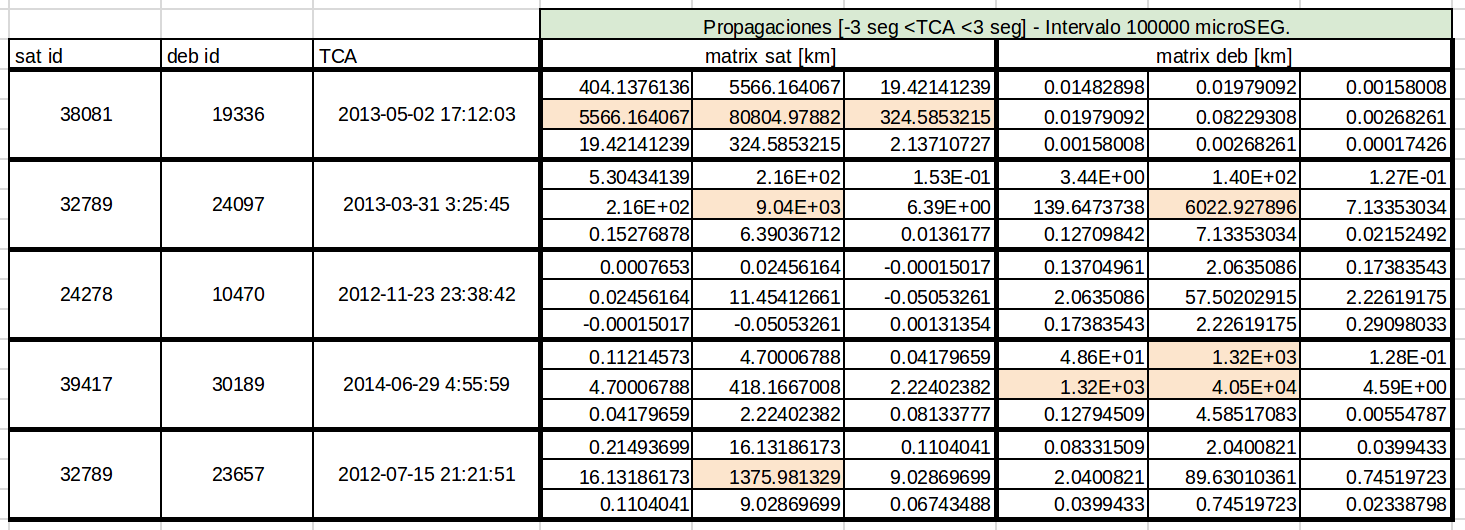
\includegraphics[width=\textwidth]{imagenes/tablaMAmails}}
%   \caption{Tabla con las matrices de covarianza calculadas por ARxCODE (m\'etodo de Osweiler) para la misi\'on y el desecho. Se resaltan los valores que con errores grandes}
%   \label{fig:tablaMAmails}
% \end{figure}
% 
% Se observa, que las matrices calculadas para introducir en el c\'alculo del encuentro de ARxCODE, introducen errores muy grandes y los elementos de su diagonal, correspondientes a las varianzas en cada una de las componentes RTN, son mucho mayores a las que se indican en los mails.\\
% 
% De estos resultados se desprende que los valores publicados en los mails, son m\'as precisos a los que se pueden lograr con ARxCODE y seguramente han sido calculados con datos observacionales de rastreo m\'as precisos que la informaci\'on orbital que ofrecen los TLE. 

\subsubsection*{Validaci\'on con CDM p\'ublicos}

A partir de la informaci\'on de los seis CDM, se carg\'o manualmente el identificador de NORAD del sat\'elite (sat\_id), el identificador de NORAD del desecho (deb\_id), el TCA de cada situaci\'on. Se calcul\'o la m\'inima distancia y la PoC nuevamente con el m\'etodo de Lei-Chen y con pasos de propagaci\'on distintos, en un caso cada un segundo (Tabla \ref{tab:cdmsproc1seg}) y en otro caso para un paso menor, de cien mil microsegundos (Tabla \ref{tab:cdmsproc100mseg}).
 
 \begin{table}[!h]
  \caption{ARxCODE a partir de los CDM \\ Propagaciones cada 1 segundo - (Radio de colisi\'on $r_{a}=0.01$ km) - M\'etodo de c\'alculo de PoC: Lei-Chen}
 \centering
 \resizebox{17cm}{!}{
\begin{tabular}{ccrrrrr}
 \hline \hline
 \# & TCA arx & $\Delta R_{arx}$ [km] & $\Delta T_{arx}$ [km] & $\Delta N_{arx}$ [km] & Min Dist. arx [km] & PoC arx\\
 \hline \hline
 1 & 2013-01-10 09:59:57 &0.295626&1.358542&1.321294&1.918033& 1.4e-05 / 1.4e-05\\
 
 2 & 2013-01-12 00:20:51 &0.405629&4.127385&1.632732&4.457091&0.0 / 0.0\\
 
 3 & 2013-01-10 13:22:45 & 0.382972 & 1.173174  & 1.316177 & 1.804252 & 8e-06\\

 4 & 2013-01-11 05:30:56 & 0.01038& 1.276203& 0.648991&1.431779&0.0\\
 
 5 & 2012-11-22 13:03:45.0 & 0.027395 & 4.661372 & 0.332569 & 4.673301 & 1.4e-05/1.4e-05 \\
 
 6 & 2012-12-26 05:00:41 & 0.183897& 4.661359&0.02668&4.665061& 0.0 / 0.0\\
 \hline
 \end{tabular} }
 \label{tab:cdmsproc1seg}
 \end{table}
 
\begin{table}[!h]
 \caption{ARxCODE a partir de los CDM \\ Propagaciones cada 100.000 microsegundos - (Radio de colisi\'on $r_{a}=0.01$ km) - M\'etodo de c\'alculo de PoC: Lei-Chen}
\centering
 \resizebox{17cm}{!}{
\begin{tabular}{ccrrrrr}
 \hline \hline
 \# & TCA arx & $\Delta R_{arx}$ [km] & $\Delta T_{arx}$ [km] & $\Delta N_{arx}$ [km] & Min Dist. arx [km] & PoC arx\\
 \hline \hline
 1 &2013-01-10 09:59:57  &0.295626&1.358542& 1.321294&1.918033&1.4e-05 \\
 
 2 & 2013-01-12 00:20:51.3 &0.401158&0.140306&0.218037&0.477654&6.1e-05\\
 
 3 & 2013-01-10 13:22:45.2 & 0.382381 &0.288759& 0.043842&0.481165&9e-06\\
 
 4 &2013-01-11 05:30:55.9&0.016754 &0.215364 &0.573953&0.613257&0.0\\
 
 5 & 2012-11-22 13:03:44.7 & 0.023908 & 0.436662& 0.758981 & 0.875955 & 2e-05 \\
 
 6 & 2012-12-26 05:00:40.7 & 0.183162& 0.1859&0.417861&0.492661& 1.24e-04\\
 \hline
 \end{tabular} }
 \label{tab:cdmsproc100mseg}
 \end{table}

 \begin{table}[!h]
 \caption{M\'inimas distancias de acercamiento para distintos pasos de propagaci\'on \\ y resultados de los CDM. (Radio de colisi\'on $r_{a}=0.01$ km)}
\label{tab:cdmsMinD}
\begin{tabular}{lccc}
 \hline \hline
  \rowcolor{lightgray}
 \# & Dist (1 seg) [km] & Dist (100 mil $\mu$ seg) [km] & Dist. CDM\\
 \hline \hline
 1 & 1.918 &  1.918&  0.170 \\
 
 2 & 4.457 & 0.477 & 0.175  \\

 3 & 1.804 & 0.481 & 0.180\\
 
 4 & 1.431 & 0.613 & 0.150\\
 
 5 & 4.665 & 0.875 & 0.976 \\
 
 6 & 4.665 & 0.492 & 0.617\\
 \hline
\end{tabular} 
\end{table}

Para estos \'ultimos procesamientos es notoria la diferencia que se produce cuando se incrementa el paso de propagaci\'on al orden de los cien mil microsegundos; logrando as\'i que los valores calculados por ARxCODE para las m\'inimas distancias se aproximen al valor que publican los CDM.\\

No se pudo identificar a qu\'e se debe esta distinci\'on entre las mejoras que se logran en los CDM, que no se logran en la informaci\'on de los correos electr\'onicos. Probablemente se deba a la incerteza en el TCA que introducen los correos al no informar el TCA con precisi\'on del segundo.\\

\subsubsection*{Validaci\'on con escenarios que incluyen el valor de PoC}

A continuaci\'on se presentan los resultados obtenidos utilizando los tres m\'etodos descriptos  para el c\'alculo de la PoC (Sec. \ref{sec:calculoPoC}), para los diez escenarios propuestos con los valores estimados de la PoC.\\ 

Dado que el c\'alculo de la distancia se realiza en primera instancia y es independiente del m\'etodo de c\'omputo de la PoC que se utilice, en la primera tabla (Tabla \ref{tab:distlimite}) se muestran las diferencias de las distancias calculadas con las publicadas y los valores de las PoC publicadas para ser comparadas con los valores calculados con el m\'etodo del l\'imite. 


 \begin{table}[!h]
 \caption{Diferencias que resultan de comparar las distancias calculadas\\ y las PoC que se obtienen con el m\'etodo del l\'imite, respecto\\ de los valores de los casos de prueba.}
\label{tab:distlimite}
\begin{tabular}{lccc}
 \hline \hline
 \# & $\Delta$ Distancia [km] & PoC (publicada) & PoC (l\'imite) \\
 \hline \hline
1&- 0.010&1.74E-03&1.50E-01\\
2&1.583&2.62E-04&2.59E-03\\
3&0.004&1.10E-04&4.68E-03\\
4&0.082&6.10E-04&1.99E-02\\
5&0.054&2.18E-04&3.24E-03\\
6&0.201&1.55E-04&1.62E-02\\
7&0.778&1.24E-05&4.88E-03\\
8&-0.071&1.70E-06&1.30E-01\\
9&0.716&3.01E-05&5.35E-03\\
10&-0.001&1.50E-05&4.67E-02\\
 \hline
\end{tabular} 
\end{table}

Las diferencias en las distancias fueron calculadas haciendo la resta entre el valor computado por ARxCODE y el valor publicado, de modo tal que los valores positivos indican que las estimaciones de ARxCODE son mayores a las publicadas; que es lo que ocurre en la mayoría de los casos. Mientras que las diferencias negativas, indican situaciones en las cuales el valor obtenido por ARxCODE para la m\'inima distancia es menor al publicado.\\

Puede apreciarse que los valores estimados para la PoC con el m\'etodo de l\'imite ofrecen siempre valores al menos un orden de magnitud mayor al publicado. Siempre indica PoC mayores, independientemente de c\'omo resulten las distancias relativas. Esto garantiza que todos los casos que se analizaron hubieran sido alertados, de utilizarse los resultados de este m\'etodo para el criterio de generaci\'on de situaciones de riesgo. Si bien seguramente ser\'a generador de falsas alarmas, puede considerarse como un primer filtro, para colectar eventos que requieran un an\'alisis m\'as fino.\\

Tanto para el m\'etodo de Lei-Chen \citep{leichen} como para el de Akella \& Alfriend \citep{akellaAlfriend}, se incorporaron dos pruebas m\'as, con el objeto de analizar la sensibilidad de la PoC a las matrices de covarianza. Es decir, se ejecutaron ambos m\'etodos utilizando tres matrices de covarianza diferentes. En primer lugar se ejecut\'o el sistema sin modificaciones, utilizando la matriz de covarianza que genera ARxCODE con el m\'etodo de Osweiler (ma. OSW), luego se hizo una prueba que reemplaza la matriz generada por los valores que se proponen desde el servicio web SOCRATES, a saber (en el sistema RTN):

$$
 C_{SOCRATES}=
\begin{bmatrix}
    (0.1)^{2} & 0 & 0  \\
    0 & (0.3)^{2} & 0  \\
    0 & 0 & (0.1)^{2} 
\end{bmatrix}
$$

Dado que esta \'ultima matriz es del orden de los valores calculados para la matriz de propagaci\'on de errores, este caso se dividi\'o a su vez en dos: el primero, que suma la propagaci\'on de errores a la matriz de SOCRATES (ma. SOC+prop) y uno que no lo hace (ma. SOC).\\

Como puede apreciarse en las matrices que se muestran a continuaci\'on, la matriz que genera ARxCODE (Tabla \ref{tab:maOswSocrates}) contiene varianzas muy grandes, en muchos casos del orden de los cientos de metros en la direcci\'on de la componente T, que acompaña a la velocidad. Luego, las modificaciones que incorpora el m\'etodo propuesto para la propagaci\'on de errores, resultan despreciables. Mientras que la matriz que se propone desde SOCRATES, a\'un sumando la propagaci\'on de errores (Tabla \ref{tab:maSocratesprop}) se mantiene acotada, y alcanza un m\'aximo del orden de $1.5$ km para la componente T.\\

\begin{table}[!h]
\centering
\makebox[0pt][c]{\parbox{1.0\textwidth}{%
    \begin{minipage}[b]{0.48\hsize}
    \caption{Varianzas que resultan de ARxCODE\\ (m\'etodo de Osweiler)}
    \resizebox{7.2cm}{!}{
      \begin{tabular}{cccc}
	\hline
     \#  & $\sigma_{R}^{2} [km^{2}]$&  $\sigma_{T}^{2} [km^{2}]$& $\sigma_{N}^{2} [km^{2}]$\\
      \hline
      1 & 0.214 & 135.094 & 0.305\\
      2 & 0.176 & 141.451 & 0.293\\
      3 & 0.144	& 3.573	  & 0.292\\
      4 & 0.083	& 1.598	  & 0.378\\
      5 & 0.136	& 266.660 & 0.333\\
      6 & 0.242	& 516.868 & 0.322\\
      7 & 0.200	& 5.775	  & 0.557\\
      8 & 0.098	& 1.147	  & 0.286\\
      9 & 0.313	& 1710.837& 0.384\\
      10& 0.078	& 1.228	  & 0.294\\
      \hline
      \end{tabular}}
        \label{tab:maOswSocrates}
    \end{minipage}
    \hfill
    \begin{minipage}[b]{0.48\hsize}
    \caption{Varianzas de SOCRATES\\ m\'as la propagaci\'on de errores}
     \resizebox{7cm}{!}{
    \begin{tabular}{cccc}
      \hline
     \# & $\sigma_{R}^{2} [km^{2}] $&  $\sigma_{T}^{2} [km^{2}] $& $\sigma_{N}^{2} [km^{2}] $\\
    \hline
    1 & 0.126 & 1.469 & 0.298\\
    2 & 0.100 & 1.233 & 0.307\\
    3 & 0.126 & 1.469 & 0.298\\
    4 & 0.088 & 1.199 & 0.325\\
    5 & 0.126 & 1.469 & 0.298\\
    6 & 0.126 & 1.469 & 0.298\\
    7 & 0.126 & 1.469 & 0.298\\
    8 & 0.097 & 1.081 & 0.305\\
    9 & 0.111 & 1.275 & 0.302\\
    10& 0.086 & 1.039 & 0.311\\
    \hline
    \end{tabular}}
      \label{tab:maSocratesprop}
   \end{minipage}
    \hfill
}}
\end{table}

A continuaci\'on se muestran las dos tablas (Tabla \ref{tab:resulLeichen} y Tabla \ref{tab:resulakella}) con los resultados del c\'alculo de la PoC con los m\'etodos de Lei-Chen y Akella \& Alfriend respectivamente. En las diferentes columnas se distinguen los resultados de acuerdo a las matrices de covarianza utilizadas en cada procesamiento.\\

Los procesamientos realizados con la implementaci\'on del m\'etodo de Lei-Chense (Tabla \ref{tab:resulLeichen}) se apartan en uno o dos \'ordenes de magnitud de los datos publicados en todos los casos. Cuando se utiliza la matriz que construye ARxCODE mediante el m\'etodo de Osweiler, se obtienen valores de PoC menores; salvo para:\\

\begin{itemize}
 \item Caso \#7: que presenta una pequeña diferencia en el valor, pero no en la magnitud.
 \item Casos \#8 y \#10: que presentan valores mayores de PoC, como es de esperar debido a que se obtiene un valor menor para la m\'inima distancia.
 \item Caso \#1: en contradicci\'on a lo que se espera, este caso resulta en una PoC menor, siendo que la m\'inima distancia es menor. 
\end{itemize}


\begin{table}[!h]
 \caption{PoC que se obtienen con el m\'etodo de Lei-Chen para los tres casos de matrices de covarianza distintas.}
\label{tab:resulLeichen}
\begin{tabular}{lccccc}
 \hline \hline
 \# & $\Delta$ Distancia [km] & PoC (dato) & PoC (ma. OSW) & PoC (ma. SOC+prop) & PoC (ma. SOC) \\
 \hline \hline
1&-0.010&1.74E-03&1.13E-05&7.63E-05&1.42E-04\\
2&1.583&2.62E-04&1.36E-05&2.19E-05&1.07E-05\\
3&0.004&1.10E-04&2.55E-05&2.40E-05&1.23E-05\\
4&0.082&6.10E-04&1.10E-04&1.14E-04&2.00E-04\\
5&0.054&2.18E-04&1.68E-05&2.65E-05&1.49E-05\\
6&0.201&1.55E-04&1.22E-05&9.09E-05&1.56E-04\\
7&0.778&1.24E-05&2.25E-05&2.43E-05&1.43E-05\\
8&-0.071&1.70E-06&6.76E-05&6.88E-05&1.25E-04\\
9&0.716&3.01E-05&5.56E-06&5.98E-05&6.53E-05\\
10&-0.001&1.50E-05&1.20E-04&1.18E-04&2.14E-04\\
 \hline
\end{tabular} 
\end{table}

Cuando se reemplaza la matriz generada por ARxCODE por la matriz que propone SOCRATES, incluyendo la correcci\'on por propagaci\'on de errores, el comportamiento no se modifica casi nada, incluso los valores mantienen el mismo orden de magnitud.\\

Se distingue quiz\'as el caso \#9 que incrementa su valor, superando al propio valor de la publicaci\'on sin que la m\'inima distancia cambie, raz\'on por la cual no se puede aseverar que los valores siempre ser\'an menores a los publicados cuando la distancia sea mayor.\\

Finalmente, los resultados correspondientes a utilizar la matriz de SOCRATES sin la correcci\'on por propagaci\'on de errores muestran resultados an\'alogos y un incremento que supera al valor publicado en los casos \#6 y \#7.\\

Para el an\'alisis de los resultados que gener\'o el m\'etodo de Akella \& Alfriend es parece importante incorporar una columna que indique las m\'inimas distancias calculadas, ya que este m\'etodo muestra ser el m\'as sensible a la relaci\'on entre el valor de los errores y la distancia m\'inima.\\

En este an\'alisis resulta que:\\

\begin{itemize}
 \item En los casos \#4, \#6, \#8 y \#10 que tienen distancias m\'inimas menores al kil\'ometro, los resultados del m\'etodo est\'an en muy buen acuerdo con el orden de magnitud de los publicados. Si bien para los errores groseros de la matriz de Osweiler o de la matriz de SOCRATES con propagaci\'on de errores hay diferencias; en la \'ultima de las pruebas, que considera errores menores al kil\'ometro los valores se ajustan muy bien.\\
 \item El caso \#1 muestra tambi\'en un comportamiento inesperado como en el m\'etodo de Lei-Chen, no obstante tiende a crecer y a acercarse al valor publicado.\\
 \item En los casos \#2, \#3, \#5 y \#7, con m\'inimas distancias cercanas o superiores al kil\'ometro los valores de PoC son siempre muy pequeños y directamente se disparan tendiendo a cero en el caso de la matriz de SOCRATES sin propagaci\'on de errores.\\
\end{itemize}


\begin{table}[!h]
 \caption{PoC que se obtienen con el m\'etodo de Akella \& Alfriend para los tres casos de matrices de covarianza distintas.}
\label{tab:resulakella}
\resizebox{17cm}{!}{
\begin{tabular}{lcccccc}
 \hline \hline
 \# & $\Delta$ Distancia [km] & PoC (dato) & PoC (ma. OSW) & PoC (ma. SOC+prop) & PoC (ma. SOC)& Dist. min. \\
 \hline \hline
1&-0.010&1.74E-03&7.78E-06&7.61E-05&6.75E-04&0.029\\
2&1.583&2.62E-04&2.09E-06&2.79E-06&3.27E-18&1.679\\
3&0.004&1.10E-04&1.55E-05&6.39E-06&4.97E-14&0.930\\
4&0.082&6.10E-04&7.86E-05&8.53E-05&3.74E-04&0.219\\
5&0.054&2.18E-04&1.21E-10&2.05E-09&5.30E-40&1.344\\
6&0.201&1.55E-04&3.85E-06&7.58E-05&1.08E-04&0.268\\
7&0.778&1.24E-05&3.87E-07&2.15E-07&5.08E-21&0.893\\
8&-0.071&1.70E-06&7.42E-05&7.42E-05&6.56E-04&0.033\\
9&0.716&3.01E-05&1.89E-06&4.63E-05&2.17E-06&0.814\\
10&-0.001&1.50E-05&9.96E-05&1.06E-04&4.48E-04&0.093\\
 \hline
\end{tabular} }
\end{table}

\paragraph{El caso \# 1}
El caso \#1 analiza un encuentro de riesgo entre la misi\'on operativa Sentinel 1B (41456) y el desecho espacial IRIDIUM 33 (35732). Si bien este caso muestra un resultado inesperado al no lograr alcanzar o superar el valor publicado, a\'un cuando la distancia m\'inima calculada es menor que la publicada, es importante destacarlo, ya que mediante una publicaci\'on en internet de la ESA (\footnote{https://sentinel.esa.int/web/sentinel/news/-/article/sentinel-1b-collision-avoidance-manoeuvres-on-29-june-2018}) se puede comprobar que la situaci\'on condujo a una maniobra evasiva (Fig. \ref{fig:envisatRMM}). 

 \begin{figure}[H]
  \centering
  \fbox{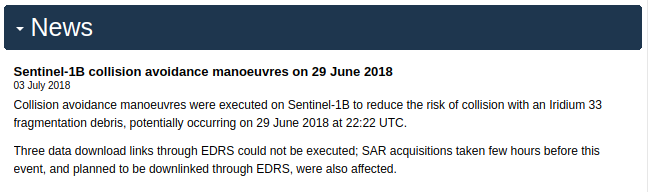
\includegraphics[width=\textwidth]{imagenes/sentinelRMM}}
  \caption{Notificaci\'on del d\'ia 3 de Julio por parte de la ESA de la realizaci\'on de una maniobra evasiva para el Sentinel 1B (caso \#1). El texto dice: {\it{{\bf{Sentinel 1B}} maniobra evasiva el d\'ia 29 de Junio de 2018. Fue realizada una maniobra evasiva por el Sentinel 1B para reducir el riesgo de colisi\'on con un fragmento del IRIDIUM 33, potencialmente estimado para el d\'ia 29 de Junio de 2018 a las 22:22 UTC}} - Luego indica los productos satelitales afectados.}
  \label{fig:envisatRMM}
\end{figure}

Cabe destacar, que de considerarse valores superiores a $10^{-04}$ para la PoC como criterio de alarma, que es un criterio muy utilizado, cualquiera de los tres m\'etodos, considerando la matriz de covarianza de SOCRATES, hubiera detectado esta situaci\'on de riesgo. 

% \subsubsection*{C\'alculo de la PoC en funci\'on del radio de colisi\'on}
% 
% Las \'ultimas situaciones; trabajos de Klinkrad \citep{Klinkrad} y Xi \& Xiong \citep{xu2014method}; que se utilizaron para comparar los resultados de ARxCODE, dan informaci\'on de los objetos involucrados y del TCA, no obstante, no se informa sobre la estimaci\'on que han hecho para el radio de colisi\'on.\\
% 
% A continuaci\'on las Figuras \ref{fig:pocvsraEsc4} y \ref{fig:pocvsraEsc5} muestran los valores de la PoC calculados con ARxCODE en funci\'on del radio de colisi\'on elegido, para los escenarios del libro de Klinkrad descriptos previamente.\\
% 
% Como puede verse, el c\'alculo de la PoC resulta muy sensible al radio de colisi\'on considerado. Se desconoce cu\'al es el radio utilizado por Klinkrad, pero puede distinguirse que en un rango de radios de $r_{a}=0.001$ hasta $r_{a}=0.03$ kil\'ometros, se ubican las soluciones de la bibliograf\'ia.\\
% 
% Se adjuntan en el Ap\'endice \ref{App2}, los gr\'aficos an\'alogos para los resultados del trabajo de Xu \& Xiong.\\
% 
%  
% \begin{figure}[!h]
%   \centering
%   \fbox{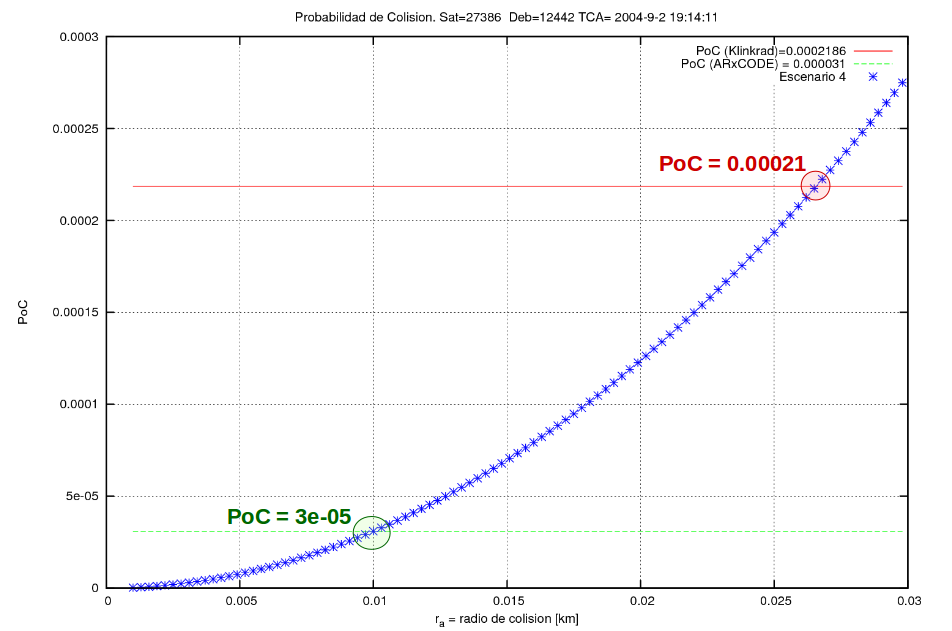
\includegraphics[width=\textwidth]{imagenes/klinkradEsc4mod}}
%   \caption{An\'alisis de la PoC en funci\'on del radio de colisi\'on. La l\'inea roja indica el valor de la PoC calculada por Klinkrad \citep{Klinkrad} y el c\'irculo se\~nala el cruce con el radio $r_{a}$ correspondiente. La l\'inea verde indica la PoC calculada por ARxCODE para un $r_{a}=0.01$ km. (Escenario 1)}
%   \label{fig:pocvsraEsc4}
% \end{figure}
% 
% \begin{figure}[!h]
%   \centering
%   \fbox{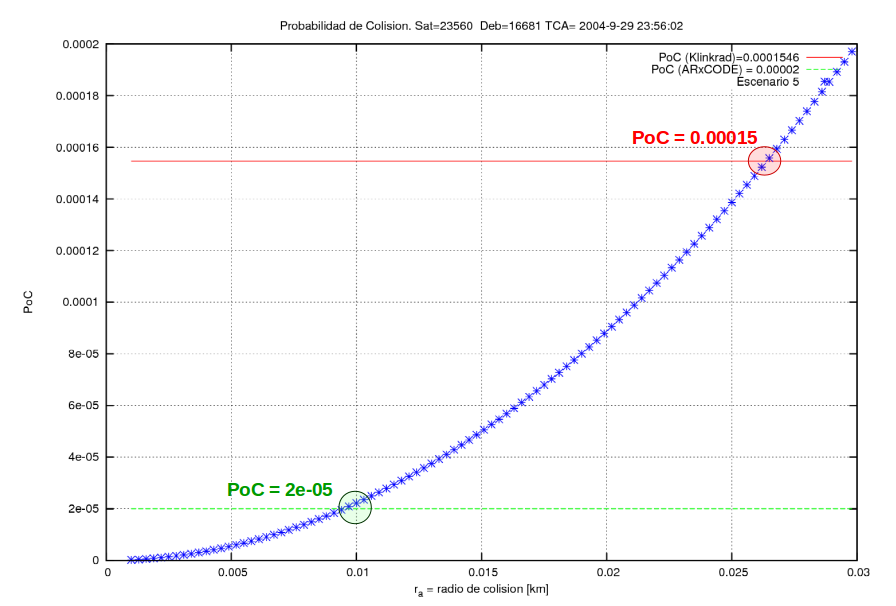
\includegraphics[width=\textwidth]{imagenes/klinkradEsc5mod}}
%   \caption{An\'alisis de la PoC en funci\'on del radio de colisi\'on. La l\'inea roja indica el valor de la PoC calculada por Klinkrad \citep{Klinkrad} y el c\'irculo se\~nala el cruce con el radio $r_{a}$ correspondiente. La l\'inea verde indica la PoC calculada por ARxCODE para un $r_{a}=0.01$ km. (Escenario 2)}
%   \label{fig:pocvsraEsc5}
% \end{figure}

\newpage
\section{An\'alisis} 
 A partir de estos resultados, se desprenden los siguientes an\'alisis:\\
 
 \begin{itemize}
  \item Las funcionalidades para la conexi\'on con NORAD para la descarga de TLE, y las propagaciones que se realizan de los mismos, funcionan correctamente.\\
  \item El m\'etodo de Osweiler \citep{osweiler} para la generaci\'on de la matriz de covarianza, resulta con diferencias del orden de los cent\'imetros respecto de los valores publicados. Diferencia  aceptable dado que las \'orbitas m\'as precisas que se consideran en este trabajo tienen errores del orden de 20 metros.\\
  \item El estudio de los errores en funci\'on de la cantidad de d\'ias que se propaguen los TLE, coincide con los resultados publicados por Osweiler \citep{osweiler} y respeta los valores esperados, de acuerdo a los efectos perturbativos y las caracter\'isticas de las \'orbitas de los sat\'elites analizados.\\
  \item Los errores que se obtienen al comparar las propagaciones de los TLE con las efem\'erides precisas a lo largo de los a\~nos 2012 y 2013, mostraron un comportamiento estable y acotado, salvo outliers, como se esperaba. Con cotas superiores de decenas de kil\'ometros.\\
  \item La metodolog\'ia utilizada para estimar errores en la propagaci\'on, mostr\'o resultados comparables a los calculados por Flohrer et al., \citep{flohrer2008assessment} y tambi\'en del mismo orden que aquellos que se sugieren en el servicio web SOCRATES.
  \item Las transformaciones al sistema de referencia RTN tienen diferencias del orden de las decenas de metros con las publicadas en el ejemplo de Lei-Chen \citep{leichen}.\\
  \item No se cuenta con datos para poder validar las proyecciones de la posici\'on relativa y la matriz de covarianza al plano de encuentro.\\
  \item Se utilizaron correos electr\'onicos de alertas y CDM que son p\'ublicos en internet para validar las diferencias que se obtienen entre las distancias m\'inimas que estos datos contienen y las distancias m\'inimas calculadas por ARxCODE. Se notaron grandes diferencias y se prob\'o modificar el paso de las propagaciones, los resultados muestran que esto no produce mejoras para los escenarios de los correos, pero los resultados de los CDM mejoran significativamente. Dado que se desconocen las situaciones iniciales de los escenarios propuestos, es probable que parte de la diferencia se deba a distintos tipos de condiciones iniciales, ya sea vectores de estado o TLE de \'epocas  diferentes a las que utiliza ARxCODE. Otro aspecto puede ser la falta de precisi\'on en el dato del TCA.\\
  \item Utilizando los mismos correos electr\'onicos y CDM se calculan las probabilidades de colisi\'on con ARxCODE, aunque el resultado no puede compararse, ya que ni los correos electr\'onicos, ni los CDM que se obtuvieron contienen esa informaci\'on. Los valores asociados a los correos electr\'onicos (que son los que cuentan con mayor diferencia en las m\'inimas distancias) dan siempre nulos en las propagaciones con pasos del segundo, y algunos resultados mejoran al achicar el paso. En cambio, en los resultados asociados a los CDM se encuentran valores aceptables en ambos casos, aunque mejores para las iteraciones menores al segundo.\\
  \item Se analizaron diez casos de prueba que contienen el dato de la PoC: cuatro casos publicados mediante el servicio web de SOCRATES \citep{Kelso} que ofrece Celestrack (Tabla \ref{tab:sisal}),  dos casos  presentados en el libro de Klinkrad \citep{KlinkradChapter8} y cuatro casos publicados en un trabajo de Xu-Xiong \citep{xu2014method}. Se calcularon las m\'inimas distancias para los diez casos y las diferencias con los valores publicados seg\'un el caso. Al igual que para los CDM y los correos electr\'onicos las diferencias resultaron significativas, y probablemente dependa de la utilizaci\'on de condiciones iniciales diversas. 
  
  \item Se calcul\'o la PoC para los diez casos de prueba mencionados en el p\'arrafo anterior. Cada caso se proces\'o con los tres m\'etodos propuestos: m\'etodo del l\'imite, m\'etodo de Lei-Chen y m\'etodo de Akella \& Alfriend. Los \'ultimos dos m\'etodos se probaros a su vez, utilizando tres matrices de covarianza diversas en cada caso, para evaluar la sensibilidad de la PoC a los errores. Los valores que devuelve el m\'etodo del l\'imite sin duda son una cota muy amplia que s\'olo puede considerarse como un primer filtro, no obstante se corre el riesgo de generar demasiados casos con falsas alarmas. El m\'etodo de Lei-Chen, por el contrario siempre ofrece valores m\'as pequeños de PoC que los publicados, esto es un riesgo ya que descarta situaciones de riesgo, aunque su respuesta mejora significativamente cuando se reducen los errores utilizando la matriz de SOCRATES. El m\'etodo de Akella \& Alfriend muestra un comportamiento similar al de Lei-Chen, pero cambia radicalmente su respuesta cuando los errores considerados son peque\~nos y/o las distancias involucradas son muy grades, en la misma direcci\'on ajusta mucho mejor el valor de la PoC para errores y distancias peque\~nas.\\
  
 \end{itemize}
